\chapter{State Consistency}
\label{chp:CONSISTENCY}

Key to designing an MMVE is to design its state consistency architecture. On a physical level, each computer that executes a virtual environment (VE) is executing a copy of the virtual environment. This is because a computer can only operate on what is stored in its primary memory. Because computers cannot access each other's primary memory banks, the necessity of multiple object copies is created.

A virtual environment can be characterised by its state. The \emph{environment state} (\emph{game state} when the environment is an online game) includes all positions, health and other attributes of all avatars, NPCs and other objects in the VE. The environment state consists of a collection of objects. An NPC as well as an immutable plant are both examples of objects that together make up the environment state.

When discussing how to segment VE state, it is sometimes easier to speak in terms of \emph{objects}, since they are separable. For the purposes of this work, objects are entities with both state and logic, which means they consume both storage space, as well as computing resources. Objects can also produce events, which should be sent to other objects. When this definition is used, NPC objects may be classified as a specific type of object, which forms part of the global game state.

The existence of multiple object copies necessitates an object consistency model. In MMVEs, each computer uses the information of the virtual environment, stored in memory, to display the virtual environment to the user. The user makes decisions based on what is displayed and the executed operations on the environment. These operations can effect change in the environment and this change has to be communicated to all other entities capable of interacting with the environment. The fact that users operate on a local version of the environment and that the environment should appear the same to all users requires state consistency mechanisms.

\section{Event-logic-update cycle}
\label{event_logic_update}

It is however impossible for multiple object states to always be consistent, because it takes time to send a message about an object update that has occurred. It is, therefore, not a good design to allow objects to be locally changed and those changes to then be communicated to other objects, because other objects may also have been locally changed in a way that would not allow for the change in the first object.

An example would be of one player in a virtual game world dealing five damage to another player with five health. When the damage is dealt, the target player is killed. If, however, the player drank a potion that gives it some health, the damage dealt by the first player would not kill him. The state of the player being dead and the player being alive is not possible at the same time.

To overcome this difficulty, a disconnect is introduced between the actions that can be performed on objects and the effect that the actions can have on objects. This is called the event-logic-update cycle \cite{}.

\emph{Events} are generated by objects and can be thought of as actions taken by agents, where agents can be humans or artificial intelligence (AI) scripts. These include casting a spell, using an item or walking.

\emph{Environment logic} is applied to events to determine what updates should be applied to the environment state. Environment logic is thus a ``think'' function, which determines how the environment should change as a result of an event. Another way to think about environment logic is to see it as the game rules.

A player casting a spell might cause another player's health to be reduced, her own health to be increased or a monster to spawn. When a player is walking, the logic will cause the player's position to update at the player's walking speed.

Environment logic communicates how the world should change via \emph{state updates}. State updates are the incremental changes that specify how the environment state should change.

An object exists in two forms: the authoritative object and the non-authoritative object. The state of the authoritative object is considered to be the true state or absolute state. Copies of the authoritative object can be made, but these copies are all non-authoritative objects. If a discrepancy occurs between an authoritative object and a non-authoritative object, the state of the authoritative object is considered to be the true state. The work of the consistency mechanism in the VE is to ensure that all non-authoritative object states follows the authoritative object state within a time frame that is reasonable for the particular VE and the particular type of object.

Authoritative objects are the objects traditionally housed on the server in the C/S based MMOGs. All clients obtain replicas of these objects and duplicate them locally in order to perform low latency computations. An example would be an NPC monster. When players perceive the monster in the virtual world, a duplicate of the NPC objects is sent to the user's computer for display purposes. When another player attacks the NPC, the change in health will be computed at the server and an update is then sent in order to ensure consistency between root and replica objects.

\begin{figure}[htbp]
 \centering
 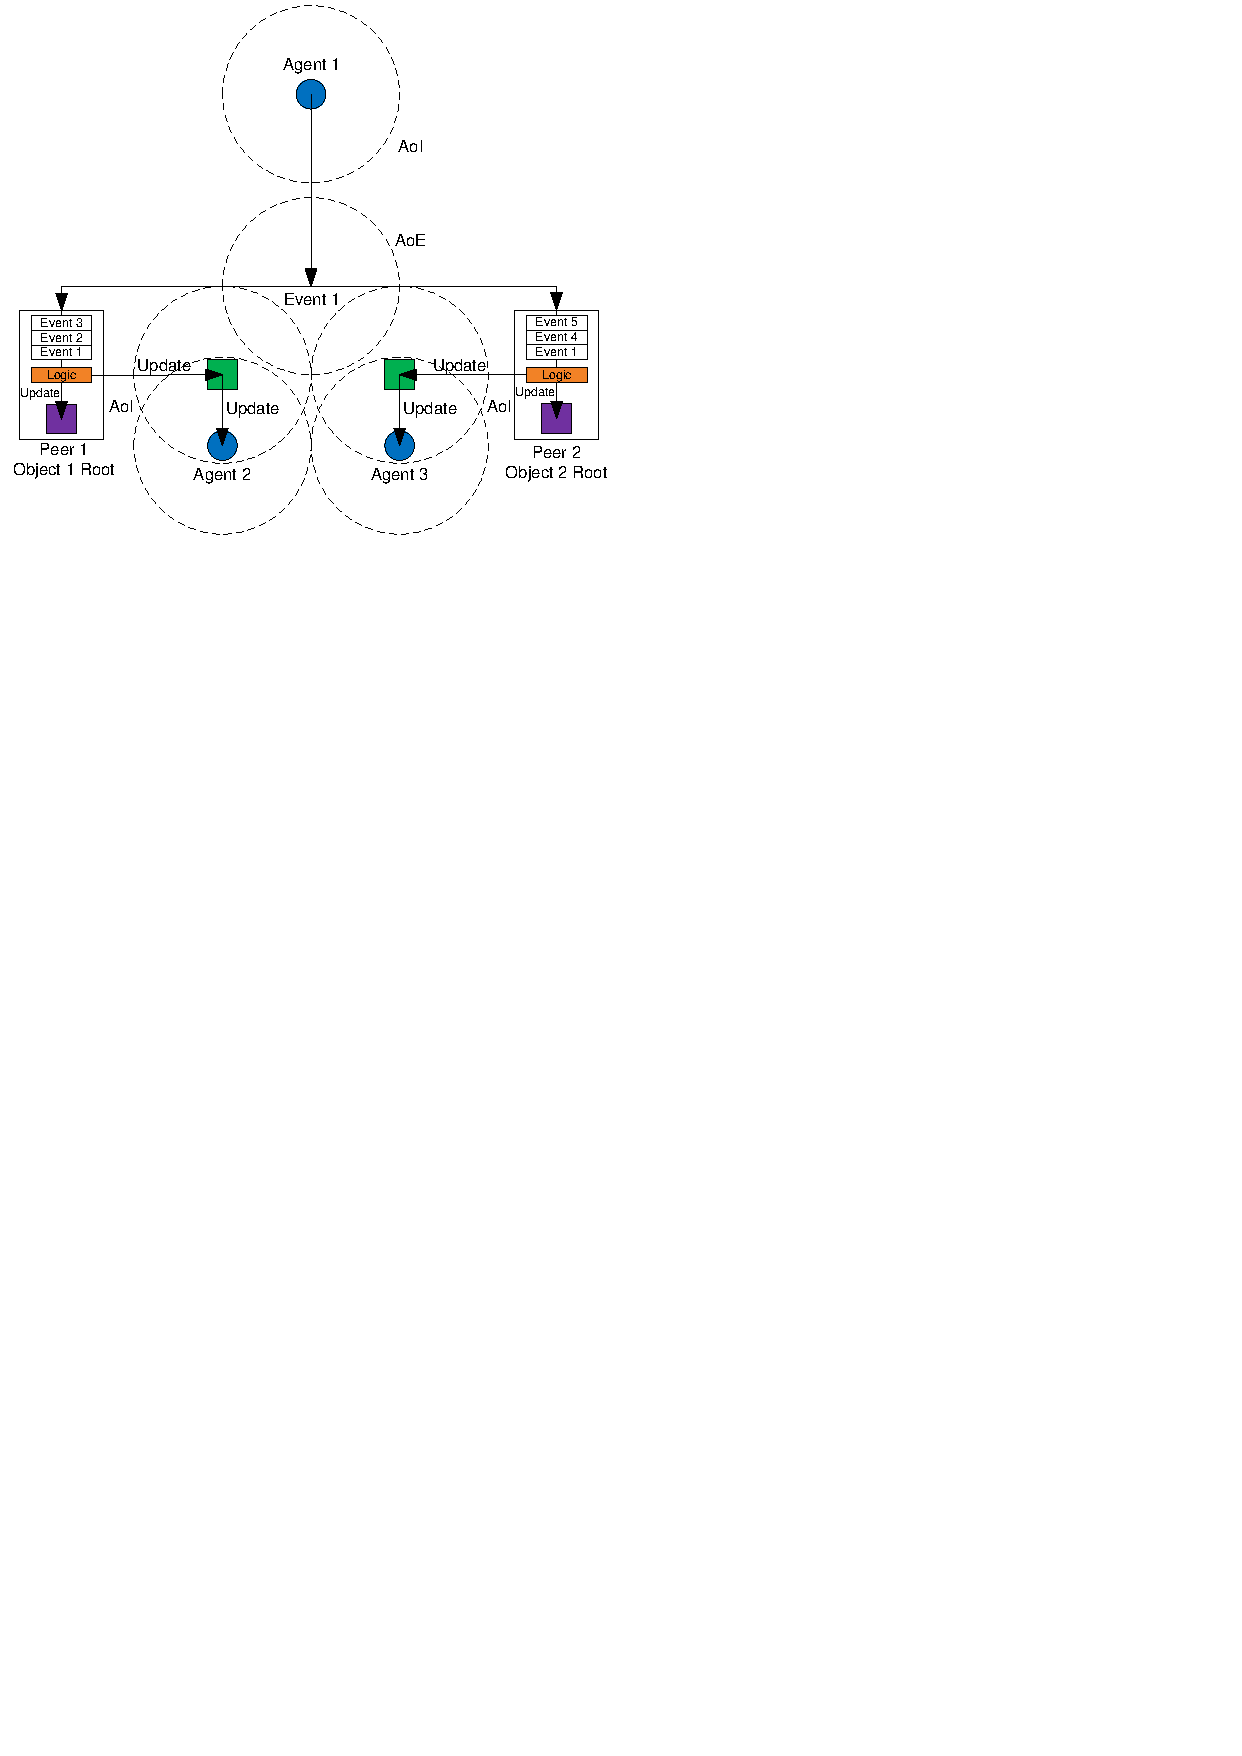
\includegraphics[clip=true, viewport=0cm 20.5cm 10.5cm 30cm, width=0.8\textwidth]{generic_consistency_graphic}
 \caption{Graphic showing the flow of events and updates to achieve state consistency}
 \label{fig_event_update_flow_graphic}
\end{figure}

Figure \ref{fig_event_update_flow_graphic} depicts the flow of events and updates in response to the generation of an event by some agent. Agents are defined to be some form of intelligence that can interact with the virtual environment. An agent can either be a human or an artificial intelligence script driving some object in the VE.

In Figure \ref{fig_event_update_flow_graphic}, Agent 1 generates Event 1 at the remote location shown. To maintain generality, events are defined to possess areas of effect (AoEs). An event's AoE determines which objects are in range to be potentially affected by an event. When an event's AoE encloses an object, that object is in range to be affected by the event. Whether the object is affected by the event, will be determined by the game logic.

In Figure \ref{fig_event_update_flow_graphic}, Event 1 affect Object 1. Event 1 is, therefore, sent to Object 1's root node, i.e. the peer housing the authoritative copy of Object 1. Determining which objects are affected by an event is termed \emph{event layer interest management}. Delivering the event to the root nodes of the affected object is termed \emph{event dissemination}.

When Event 1 arrives at Peer 1, containing Object 1, the event is placed in a event queue in an order based on the time each event occurred. The process of determining which order events have to be processed in is called \emph{event ordering}. Many events will be arriving at an object's root node from multiple agents simultaneously.

After event ordering has been performed, environment logic is applied to determine hoe a specific event will affect a specific object. To determine possible updates, that state of other objects might also have to be taken into account. An example is firing at a player through a wall. If the thickness of the wall determines how much damage is delivered to the player, the root node processing the damage to the player object will have to know the thickness of the wall.

When an event has been translated into a state update, the root object on the root node is updated. The new state of the object should also be communicated with all agents that can perceive the object in the virtual world. An object is perceived by an agent if the agent's area of interest (AoI) encompasses the object. Determining which agents should receive objext state updates is termed \emph{update layer interest management}. In the figure, Object 1 is perceived by Agent 2. Peer 1 therefore has to send an update to the peer housing agent 2. Delivering state updates to the affected agent peers is termed \emph{update dissemination}.

When the update is delivered to Agent 2, the local object state is updated and the object's new state is displayed to the agent to allow the agent to make decisions and, therefore, generate events based on the new object state.

\section{Classic consistency models}
\label{classic_models}

As an introduction to consistency models, an overview of the two common models, currently used in computer games will be described. The models used
in P2P MMOGs are all permutations of these two basic models. The two models are based on the two different network models. These are the fully
distributed model, also called the event-based model \cite{p2p_cm_aoe}, and the C/S-based model, also called update-based model
\cite{unreal_networking}.

\subsection{Event-based (Fully distributed)} \label{classic_cs_event_based}

\begin{figure}[htbp]
\centering \subfloat[Event-based (fully distributed)]{\label{fig_p2p_cm}
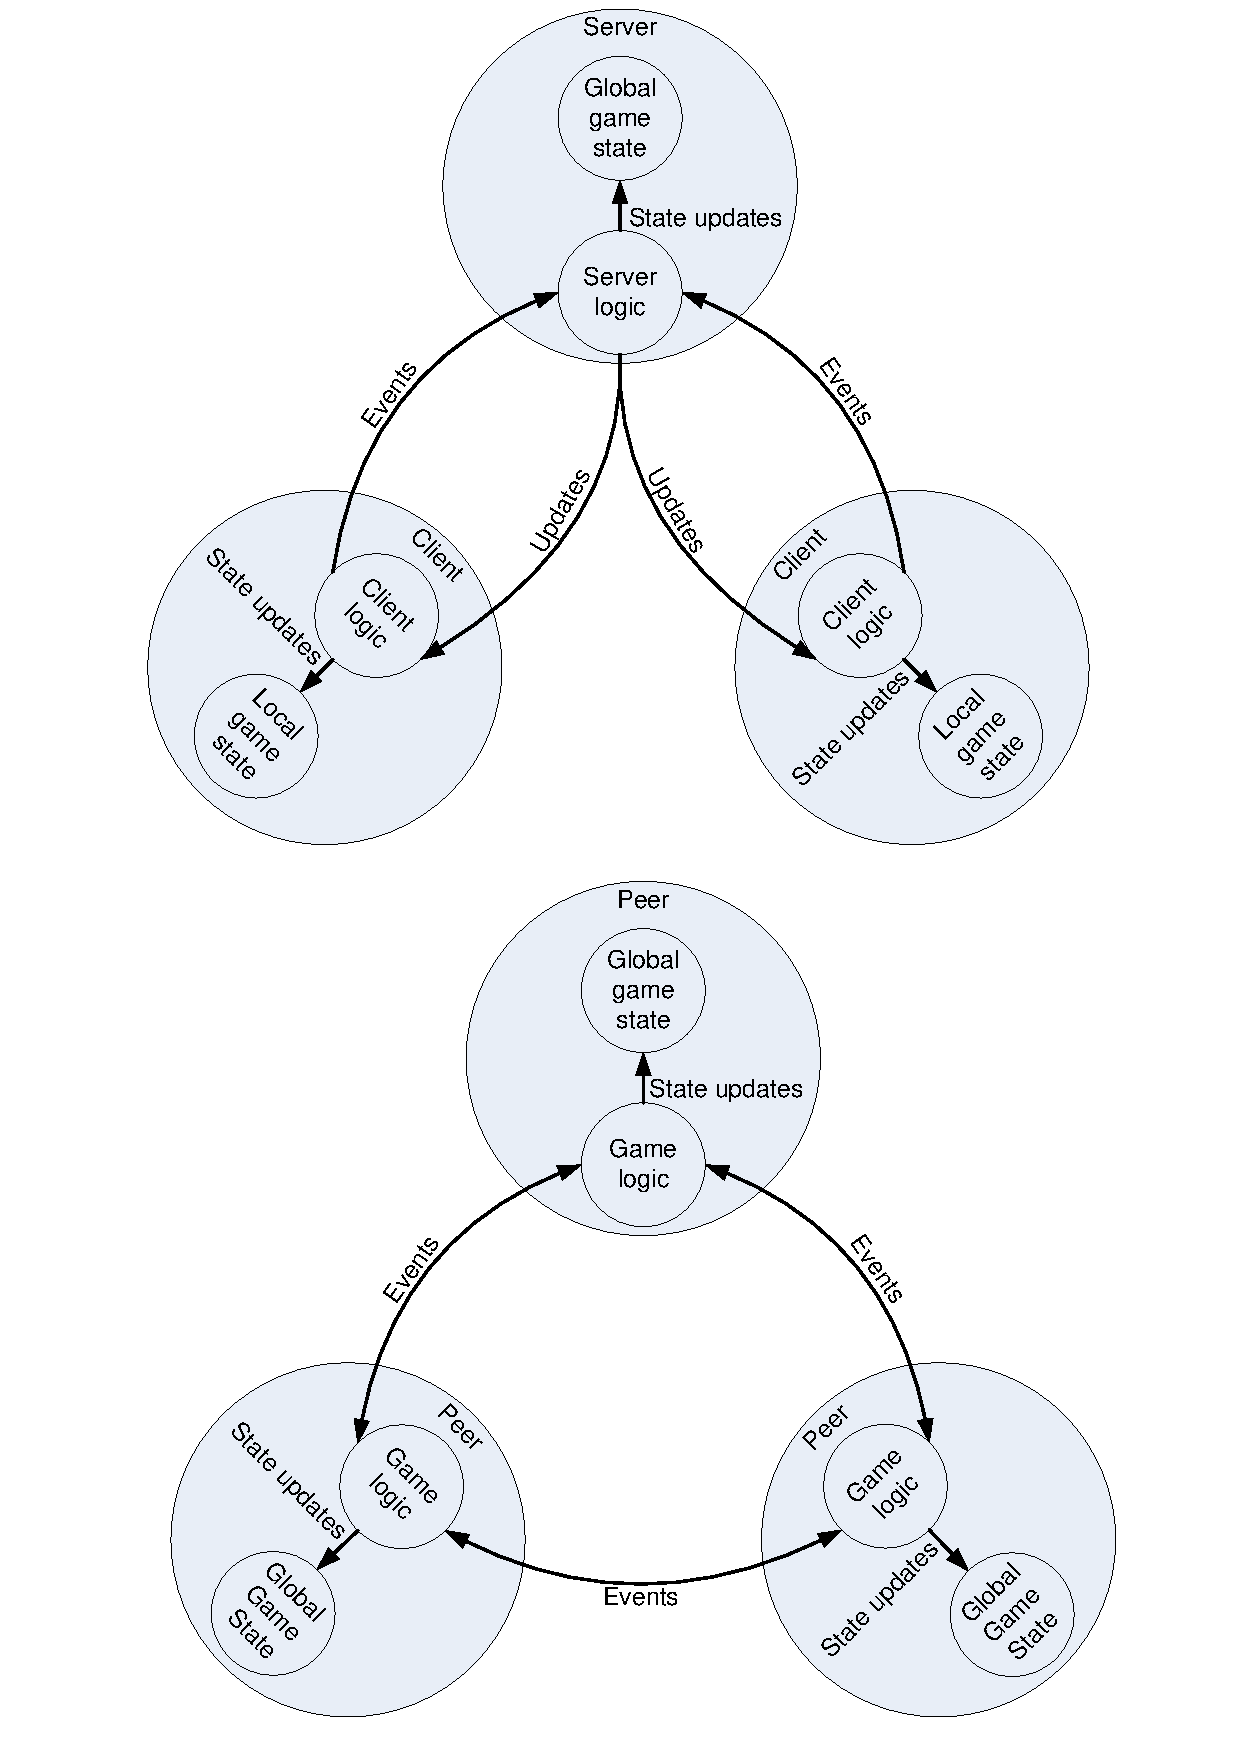
\includegraphics[clip=true, viewport= 2.5cm 0.5cm 19cm 15cm, width=\columnwidth]{CS_P2P_CMs}}
 \subfloat[Update-based (client/server)]{\label{fig_cs_cm}
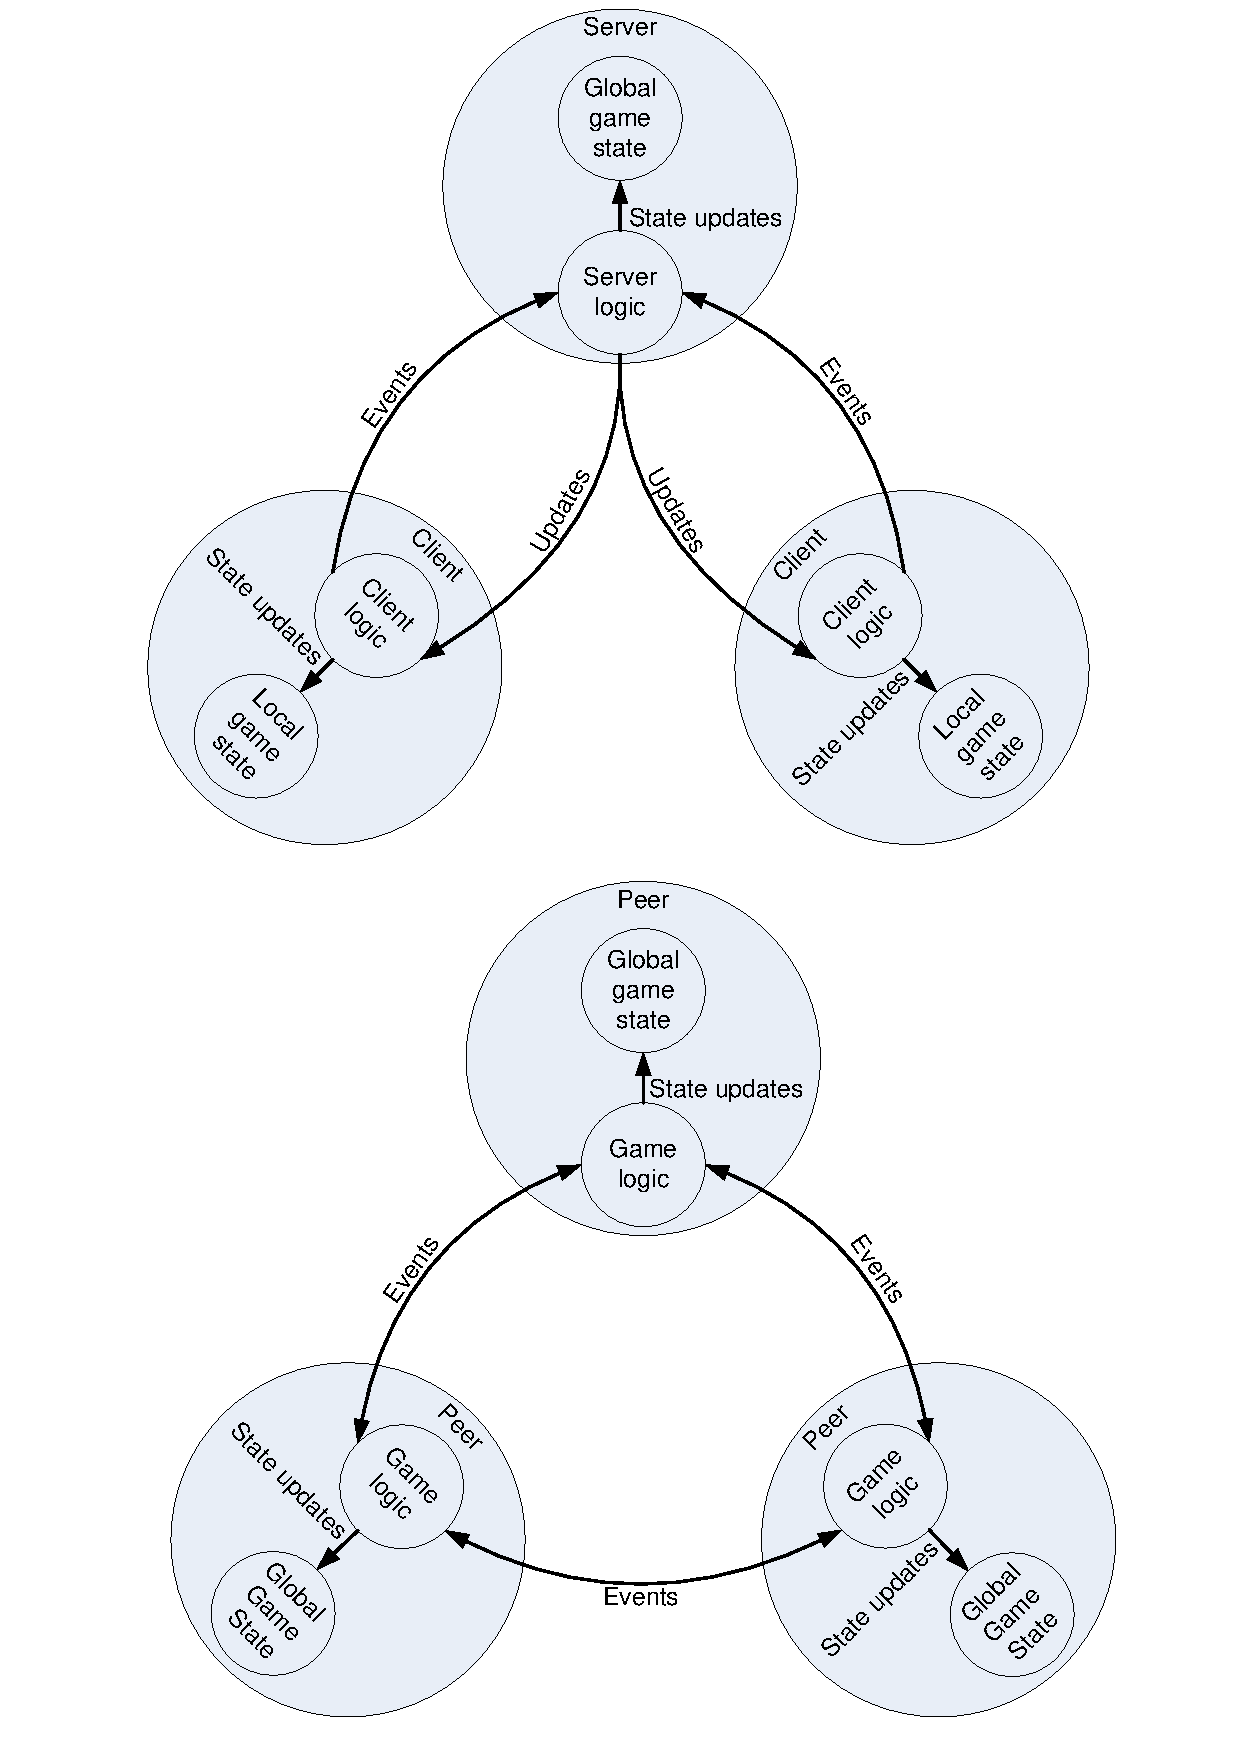
\includegraphics[clip=true, viewport= 2.5cm 15cm 19cm 30cm, width=\columnwidth]{CS_P2P_CMs}}
\caption{Consistency models}
\end{figure}
%
Figure \ref{fig_p2p_cm} shows the fully distributed model. The state persistency model for this consistency model is that the complete game state is
stored on each peer. Any event that a peer generates is sent to all other peers. These events are used as inputs to the game logic, which creates
updates, which are then used to update the global game state at each peer. The event-based model works well for strategy games, and was implemented
in Age of Empires \cite{p2p_cm_aoe} and Starcraft \cite{starcraft_network_model}.

The order in which events are received should be the same for all peers, otherwise the game states of different peers may become inconsistent.
Usually some kind of lockstep technique is used to solve this issue \cite{pessimistic_lock_step}. The issue with lockstep is that it reduces the
latency to twice that of the peer with the highest latency. Various techniques have been proposed that improves the latency by introducing some
deadline before which all events should be submitted \cite{cheat_proof_event_ordering}. This, however, makes it impossible for a player with a high
latency to play the game with anyone other than from her own continent. When latencies issues are not present and all players possess reasonable
latencies, the event-based model can provide for an high-degree of responsiveness, because of no extra latency being added by a server and no extra
server hop required for communications.

The issue with the event-based model is that it is not scalable, since all peers should connect to all other peers and every event is transmitted to
everyone. This means that as $N$, the number of peers in the network increases, the traffic increases with a factor of $N^2$. The security issues of
the P2P network model, on which this consistency model is based, are also present. Slowdown is also experienced by all players if one player's
latency is below par, since the lockstep mechanism has to wait for all events to be received for that round to conclude.

\subsection{Update-based (C/S)}

An alternative to the event-based model is the update-based model, shown in Figure \ref{fig_cs_cm}. This model is based on the C/S network model. The
persistency model here is that an authoritative global game state is housed on the server and a non-authoritative local game state is housed on all
clients for display purposes. No real game logic is housed at the clients, only on the server. All clients send events to the server, which applies
the game logic and sends updates to the clients, while also updating its own game state.

This approach greatly assists with security, as clients cannot influence the state of any other clients and every client's state depends on updates
received from the server. The server state is also termed authoritative, because if there is a conflict, the server state is always the state to
which the system is expected to return. All the security advantages of the C/S model also apply to this consistency model. Another reason why the
update based model is successful is because it is more scalable then the fully distributed model. More hardware can be used to build a more powerful
server, which can handle more clients. Computer clusters and large server are, however, costly to obtain and maintain.

The update-based model is used in many, if not all, MMOGs currently in operation. This includes games like World of Warcraft, Eve Online and Ultima
Online, to name just a few.

\subsection{Client/Multi-Server consistency models}
\label{cms_models}

%Should I add diagrams here?

Apart from the two classic models, there are also models based on the C/MS network model, which are: shard-based, replication-based, object-based and
zone-based \cite{Hu_voronoi_IM}.

\subsubsection{Sharding}

The consistency model that is exemplified by having a state persistency model where the game state (world) is duplicated over multiple servers, with
players connecting to one of these servers is termed ``sharding''. Clients are not able to interact or communicate with players on other shards,
which reduces game immersion. This method does, however, allow for a more scalable system as maximum load is fixed.

Players are not able to enter a shard if that shard has reached its capacity. In the past, this has caused unhappiness amongst players, since popular
shards could be difficult to log in to. Players are also reluctant to move to a new shard, because a lot of time is invested in their characters in
their ``home'' shard. Sharding doesn't allocate resources efficiently, as one shard may be overpopulated while another is underpopulated. For all
practical purposes, this approach is still merely a C/S approach, with players forced into a specific C/S environment.

The benefit of sharding is its ease of implementation and the reduction of content designer load. Because no inter-server communication is required
and no server migration is supported, this method greatly simplifies the server design process. Another benefit of sharding is that it allows for a
relatively small game world to support many players because of the duplication of the worlds. This reduces the load on level designers and content
designers, who now have to populate a much smaller world with content.

\subsubsection{Replication-based}
%Redundant
The replication-based model is similar to sharding, with the difference that all servers share the same duplicated game state. Each server contains
the global game state and clients connect to any one of these servers (mirror-servers \cite{mirrored_server}) or through a load distribution
algorithm to a server (proxy-servers \cite{proxy_server_dist}). Each server handles all actions from clients and updates its own database. The
servers in turn send updates to each other over a high quality link, such as fibre, to maintain database consistency at high speeds.

The problem with this system is that the world is never truly consistent and that there are no optimally chosen inconsistency obfuscation boundaries.
In other words, two players standing next to each other in the virtual world, might be on different servers and, therefore, experience two slightly
different worlds.

\subsubsection{Object-based}
%Object based
The state persistency model of the object-based consistency model equally distributes all in-game objects amongst the servers
\cite{object_based_consistency1}, \cite{object_based_consistency2}, \cite{object_based_consistency3}. For an MMOG, most of these objects are expected
to be player objects. The advantage of this method is that the system load is fixed for a certain player population and that the load is equally
distributed amongst all servers. This allows for more accurate prediction and provisioning of resources, but still does not handle transient loads
well.

Another issue is inter-server communications for this architecture. The inter-server communications are random and also more than the inter-server
communications for a region based system. The reason for this is that the number of player interactions increase with a decrease in the distance
between the players. Players playing together move together, chat and interact with NPCs together. For a region based model, all player-neighbour
interactions remain local to the server.

\subsubsection{Zone/Region-based}
%Zone-based
The state persistency model of the zone-based consistency model divides the virtual world into zones or regions, which are hosted on different
servers \cite{zone_based_stat}, \cite{zone_based_dyn}. A well known example of this model is Eve Online. Busy regions are hosted on their own
servers, while multiple quiet regions are hosted on a single server. This is termed the static region approach \cite{zone_based_stat}.

The issue of the static region approach is that it does not scale well when one region is suddenly populated with players. This type of behaviour
happens quite regularly and is known as flocking \cite{flocking}. When players find something of interest in a region, many players will flock to
that region. The solution to flocking has been over provisioning of resources to handle peak loads, which suffers from the disadvantages discussed
above. Also, if the load changes, the server has to be brought off-line in order to balance the regions.

Dynamic regions are being investigated, where regions can be dynamically shifted from one server to another, in order to balance load
\cite{zone_based_dyn}. This approach adds overhead and significant complexity with regards to the migration of the data and the handling of player
actions while the data are in transit.

\section{Generic state consistency architecture}
